Machine learning is a sub-field of \gls{AI} within the broad category of
computer science. The goal of \gls{AI} is to create computer systems that
respond to their environment according to some set of criteria or goal. For
example, self-driving vehicles have computers on board that learn to avoid
curbs and humans. It is common knowledge that the use of \gls{AI} has been
expanding at a rapid rate in recent years. News stories of major tech
companies' \gls{AI} advancements are frequent and news articles abound with
data on which jobs will be replaced with \gls{AI} in the near future. 

While its use has been increasing in the commercial sector, there is also much
anecdotal evidence to support the existence of a rapid increase of \gls{AI} use
in academic research across many disciplines beyond robotics. \gls{AI} systems
have been used in detection (e.g., fraud or spam), medical diagnostics, user
analysis (e.g., Netflix ratings), and a host of scientific disciplines that
have increasing amounts of multivariate data.

Much of the recent advances to the field of \gls{AI} have occured in the
statistical realm, which forgoes domain knowledge in favor of large data sets.
Thus, machine learning and statistical learning has become somewhat of a
separate field \cite{changingml}. Machine learning research focuses on the
underlying algorithms using mathematical optimization, methods for pattern
recognition, and computational statistics.  As an application, however, this
study is not concerned with computational time, but rather the ability to
correctly predict values and categories relevant to the nuclear forensics
mission. This restricts the relevancy of the algorithms to the underlying
theory and its impact on the resulting model's accuracy. 

Machine learning algorithms can be separated into two main categories:
unsupervised and supervised learning.  The former groups or interprets a set of
input data, predicting patterns or structures. The latter includes both the
input and output data, enabling the trained model to predict future outputs.
Broadly speaking, the unsupervised learning algorithms are designed for
clustering data sets or dimensionality reduction (i.e., determining some subset
or linear combination of features most relevant to the input data) of data
sets.  Supervised learning algorithms predict both discrete and continuous
values via classification and regression, respectively. Some algorithms can
perform both classification and regression, and neural networks can even be
modified to perform either supervised or unsupervised learning. 
%Additionally, various algorithms can be strung together, which is referred to
%as \textit{ensemble methods}. One common way of doing this is performing
%deimensionality reduction prior to supervised learning
\\
\begin{figure}[!htb]
  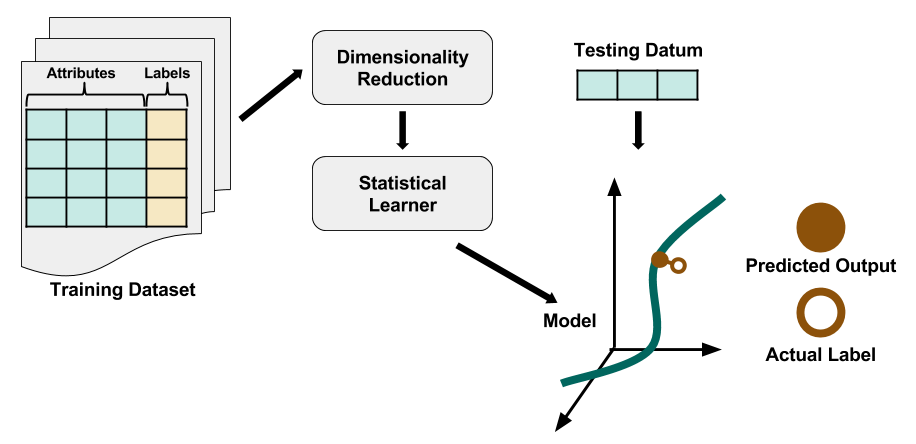
\includegraphics[width=\linewidth]{./chapters/intro/SupervisedRegression.png}
  \caption{Schematic representing a statistical learning regression algorithm}
  \label{fig:supervised}
\end{figure}

As shown in Figure \ref{fig:supervised}, a typical (supervised) machine
learning workflow begins with a training data set, which has a number of
\textit{instances}, or rows of observations.  Each instance has some
\textit{attributes}, also referred to as \textit{features}, and a label, which
can be a categorical label or discrete/continuous values.  

The training data are then inserted into a statistical learner; this calculates
some objective, minimizes or maximizes that objective, and provides some model.
This model is typically evaluated using a testing set that has the same set of
attributes and labels (but different instances). The comparison of what the
model predicts and the actual label gives the \textit{generalization error}.
Depending on the performance and application, the model may need improvement
from more training and/or some changes in the algorithm parameters. Once the
model is performing well enough and validated, it is finalized; then a user can
provide a single instance and a value can be predicted from that. 

This study performs regression tasks using supervised learning algorithms.
Differences among the underlying mathematics of the algorithms impact the
trained models.  Therefore the algorithms used in this study will be discussed
in Section \ref{sec:algs}. Next, model selection and assessment is covered in
Section \ref{sec:selectass}.  Evaluating and optimizing algorithm performance
is discussed in Section \ref{sec:optvalid}, as well as robustly comparing
different algorithms for validation.

\subsection{Algorithms for Statistical Learning}
\label{sec:algs}
\setlength\abovedisplayskip{2.5pt}

For relevant nuclear forensics predictions, both classification and regression
algorithms must be used.  For example, one may want to predict the reactor type
based on some measurements (referred to as features) of spent fuel of an
unknown source, and this would require a classification algorithm. Or perhaps
the input fuel composition is relevant to an investigation on weapons intent,
so a regression algorithm would be used to train a model based on some set of
features.  Since this work trains models to predict burnup of \gls{SNF}, the 
algorithms are presented in a regression context.

\subsubsection{Linear Models}
\label{sec:linear}

One of the simplest and most utilized methods of prediction is a linear model
from a least-squares fit. Thus, it is the most natural place to begin a
demonstration of machine learning algorithms. Since linear models must have all
parameters linearly related, there are many restrictions regarding the shape of
the model. However, this makes the resulting models stable to peturbations. 

\begin{figure}[!htb]
  \centering
  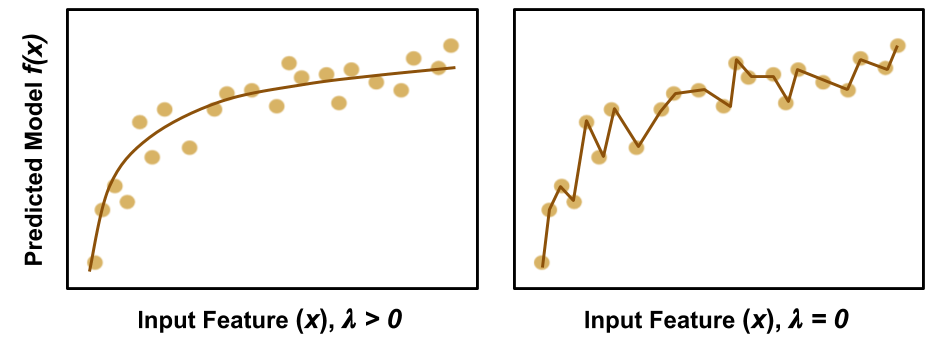
\includegraphics[width=\linewidth]{./chapters/litrev/regularization.png}
  \caption{Illustration of the effect of regularization on model prediction}
  \label{fig:reg}
\end{figure}

An example of a linear model is below, where the vector of input features of
size $p$, $\boldsymbol{X}$, provides a model, $F(\boldsymbol{X})$ ($Y$ is the
known model), by determining the unknown coefficients, or weights,
$\beta_{j}$'s. The algorithm calculates these by minimizing the value of a loss
function over all the training data.  This is usually the least squares error
from minimizing the sum of squared errors, $\sum_{i=1}^{n} (y_i - f(x_i))^2$.
But it could instead be the least absolute deviations from minimizing the sum
of absolute error differences, $\sum_{i=1}^{n} |y_i - f(x_i)|$. These are
referred to as the $L_2$ and $L_1$ norms, respectively.  
\begin{equation}
  F(\boldsymbol{X}) = \beta_{0} +  \sum_{j=1}^{p} x_{j} \beta_{j}
\end{equation}

The form of linear regression used here is called ridge regression. This
algorithm performs optimization using the $L_2$ norm, and also uses the form of
the $L_2$ norm for \textit{regularization}. Regularization, sometimes called
\textit{shrinkage}, is a term introduced into the predicted model to prevent
overfitting. (It is used in many machine learning algorithms.) This works by
further reducing the weights, $\beta_j$, on the input features, $x_j$. This
shrinkage term also includes a complexity parameter, $\lambda$
\cite{elements_stats}.  Thus, the predicted linear model from ridge regression
is updated to the following equation.  A visualization of what this
regularization can accomplish is in Figure \ref{fig:reg}.
\begin{equation}
  F(\boldsymbol{X}) = \beta_{0} +  \sum_{j=1}^{p} x_{j} \beta_{j} + \lambda \sum_{j=1}^{p} \beta_{j}^2
\end{equation}

\subsubsection{Nearest Neighbor Methods}
\label{sec:neighbor}

Nearest neighbor regression is considered to be `model-free' in that it does
not actually generalize; it tracks the observations in the training set.
During prediction, the algorithm will calculate a value based on the instance
that is closest to the current test sample. Thus, there is not any learning,
but instead a direct comparison between an unknown sample and the space that
the training set populates. The predictions from nearest neighbors can be quite
accurate, but are highly unstable to peturbations \cite{elements_stats}.  

\begin{figure}[!htb]
  \centering
  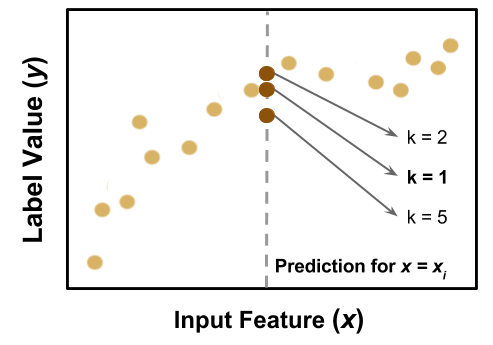
\includegraphics[width=0.8\linewidth]{./chapters/litrev/nn-fig.png}
  \caption{Schematic demonstration of regression using \textit{k}-nearest neighbors}
  \label{fig:nn}
\end{figure}

An extension of nearest neighbor is \textit{k}-nearest neighbor regression.
The closest \textit{k} neighbors are averaged to provide an estimate of the
unknown sample as shown in the equation below.  Figure \ref{fig:nn} provides a
pictoral explanation of how this is done for a single prediction.  The equation
below shows how this algorithm does this to determine a predict a value, $Y$,
from the input features, $\boldsymbol{X}$, in the neighborhood, $N_k
(\boldsymbol{X})$ \cite{elements_stats}. 
\begin{equation}
  Y(\boldsymbol{X}) = \frac{1}{k} \sum_{x_i \in N_k(\boldsymbol{X})} y_i
\end{equation}

A measure of distance dictates what the neighborhood is. The metrics for
distance differ, but in this study, the Euclidian distance was used. Another
parameter is the population of the neighborhood, \textit{k}. In this initial
work, $k = 1$ is used. This can perform very well, but can also easily overfit
the data and thus not generalize well. 

\subsubsection{Support Vector Machines}
\label{sec:svm}

\Gls{SVR} is an extension of the popular classification algorithm, \gls{SVM}.
This algorithm was chosen because of its ability to handle highly dimensional
data well, which in this study is a maximum of approximately 300 features. 

\begin{figure}[!htb]
  \centering
  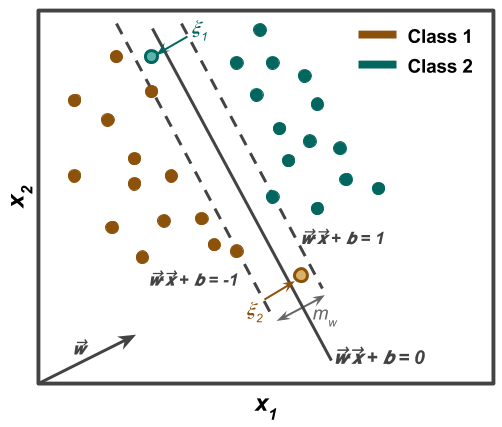
\includegraphics[width=0.8\linewidth]{./chapters/litrev/svm.png}
  \caption{Schematic demonstration of classification using SVM}
  \label{fig:svm}
\end{figure}

As seen in Figure \ref{fig:svm}\footnote{This schematic is based on the
tutorial on SVMs by Dr.\@ Saed Sayad at
http://www.saedsayad.com/support\_vector\_machine.htm}, the \gls{SVM} algorithm
separates two classes by determining an optimal hyperplane between them.  The
algorithm evaluates the quality of the line that separates the two classes by
maximizing the margin width, $m_w = \frac{2}{\lVert w \rVert}$.  The hyperplane
is defined in the equation below, where $\boldsymbol{w}$ is the vector that is
normal to the hyperplane.  
\begin{equation}
  \boldsymbol{w \cdot x} + b = 0
\end{equation}

Figure \ref{fig:svm} also shows a case of soft margins.  Some problems are not
linearly separable, and thus a penalty term, $\xi_{i}$, is introduced to allow
for some misclassifications.  The algorithm then simultaneously minimizes the
misclassifications while maximizing the margin. The objective function of the
algorithm below shows this as well (using quadratic programming). In the
equation below, $C$ is responsible for the margin width/misclassification
tradeoff.
\begin{equation}
\begin{split}
  min\ & \frac{1}{2} \lVert w \rVert ^{2} + C \sum_{i} \xi_i \\
  subject\ to:\ \ & y_i (w x_i + b) > 1 - \xi_i
\end{split}
\end{equation}

Figure \ref{fig:svr}\footnote{These schematics are based on a tutorial on SVR
by Dr.\@ Saed Sayad at
http://www.saedsayad.com/support\_vector\_machine\_reg.htm} demonstrates how
\gls{SVM} can be altered slightly from classification to nonlinear regression
with \gls{SVR}.  \Gls{SVR} has a similar objective function but instead
\textit{minimizes} the margin, as shown in Figure \ref{fig:svr-a}. This changes
the constraints to the objective function as below:
\begin{equation}
\begin{split}
  min\ & \frac{1}{2} \lVert w \rVert ^{2} + C \sum_{i} \xi_{i} \\
  subject\ to:\ \ & \lvert y_i - (w x_i + b) \rvert \leq \varepsilon + \xi_i
\end{split}
\end{equation} 

Further, this can be extended to nonlinear analysis via what is called the
\textit{kernel trick}.  First, using a nonlinear kernel function maps the data
into higher dimensional feature space. Then the algorithm can find a linear
separation in this space, as shown in Figure \ref{fig:svr-b}.

\begin{figure}[!hp]
  \centering
  \begin{subfigure}[h]{0.8\linewidth}
    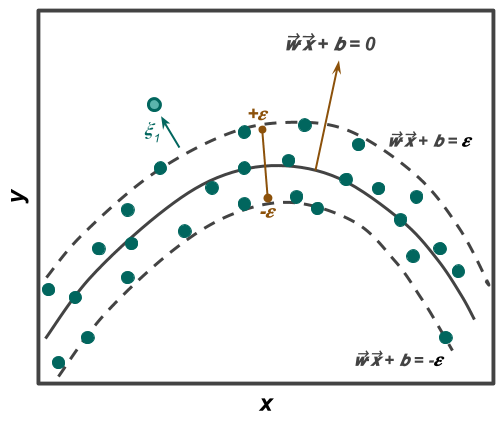
\includegraphics[width=\linewidth]{./chapters/litrev/svr-a.png}
    \caption{Demonstration of regression with \gls{SVR}}
    \label{fig:svr-a}
  \end{subfigure}
  \begin{subfigure}[h]{0.8\linewidth}
    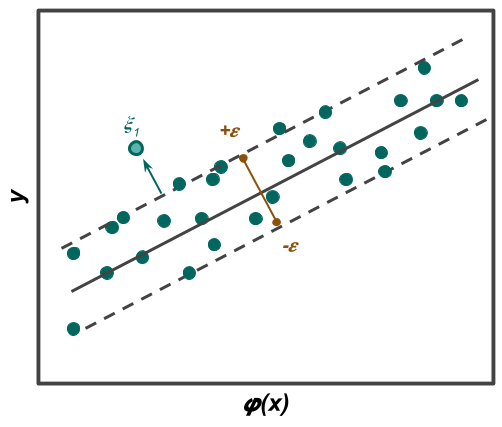
\includegraphics[width=\linewidth]{./chapters/litrev/svr-b.png}
    \caption{The kernel trick with \gls{SVR}}
    \label{fig:svr-b}
  \end{subfigure}
  \caption{Illustrations of how \gls{SVM} can be extended to both regression and nonlinear analysis}
  \label{fig:svr}
\end{figure}

The kernel chosen for this study is the Gaussian radial basis function, shown
below. This has two tuneable parameters, $\gamma$ and $C$. The $\gamma$
controls the width of influence of individual training instances, which
strongly affects the fitting of the model. Low values correspond to
underfitting because the instances have too large of a radius (low influence)
and high values correspond to overfitting because the instances have a small
radius (high influence). 

The $C$ parameter also affects the fitting of the model by allowing more or
less support vectors, corresponding to more or less misclassification,
respectivey. A lower $C$ smooths the surface of the model by allowing more
misclassifications, whereas a higher $C$ classifies more training examples by
allowing fewer misclassifications. Thus, too low or too high of a C can cause
under- or overfitting, respectively. 

Since there is a tradeoff of fitting strength provided by both parameters, it
is common to run the algorithm on a logarithmic grid from $10^{-3}$ to $10^3$
for each parameter. If plotted on a heatmap of accuracies given $\gamma$ and
$C$, there will be a diagonal of ideal combinations that emerges. The element
with the lowest of each parameter is usually chosen. 

\subsubsection{Dimensionality Reduction Techniques}
\label{sec:dimreduc}

In addition to utilizing various algorithm parameters for regularization as
discussed above, dimensionality reduction can improve generalizability by
removing the noise of features that do not affect the regression task. This can
be thought of in the following way: shrinkage techniques reduce the weights of
noisy features, whereas dimensionality reduction removes them completely.
Although one could use domain knowledge to manually reduce the number of
features in a data set (e.g., only including certain nuclide subsets such as
actinides), statistical feature reduction may also prove helpful in this work.
The mathematical treatment of the methods described below are in Ref.
\cite{elements_stats}.

%Another use for the following techniques is the visualization of one's data
%set, perhaps for data exploration or to show why certain predictions are
%difficult. 

\vspace{5mm} \noindent \textbf{Principal Components Analysis} \vspace{5mm}

\Gls{PCA} is considered the most common dimensionality reduction technique.
The \gls{PCA} algorithm learns a linear transformation of a data set
$\boldsymbol{X}$ with which to construct a transformation matrix according to a
user-chosen number of variables/components.  This matrix is part of the
singular value decomposition of the data matrix $\boldsymbol{X}$.  The
decomposition step is what provides the principal components, which are the
result of maximizing the variance in the original data while minimizing the
squared reconstruction error between the original data and the transformed
data. The mathematical assumptions are that the variables are all Gaussian and
uncorrelated.

Because the principal components are obtained purely statistically with no
model assumptions, they are usually uninterpretable. However, they can still
provide clues with which to obtain new information. In the case of this work,
this could provide insignt into new forensics signatures.

\vspace{5mm} \noindent \textbf{Factor Analysis} \vspace{5mm}

Factor analysis is similar to \gls{PCA} in that it also calculates linear
combinations of the data set features using the above-mentioned decomposition
and the mathematical assumptions are the same.  It is different in that the
decomposition is rearranged so that it represents \textit{latent variables}
including random error disturbances rather than principal components.  Latent
variables are constructed by maximizing the correlation/shared variance among
the variables rather than the total variance.  However, different optimizations
can be chosen so that the solutions are parameter-dependent.  

Furthermore, the initial model assumptions, while enabling interpretable
results, also increase the dependence of the solutions on the algorithm inputs.
If \gls{PCA} does not perform well with the type of training data in this work,
it is possible that factor analysis will, since there are many nuclides in the
training data set that are in a decay chain together.

\vspace{5mm} \noindent \textbf{Independent Components Analysis} \vspace{5mm}

\Gls{ICA} has characteristics of both factor analysis and \gls{PCA}, but with
the goal of finding independent measurements from multiple `sources'.  It uses
the same form of decomposition as factor analysis but without the inclusion of
random error. The mathematical assumptions are a bit different: the variables
are statistically independent and non-Gaussian.  This allows the algorithm to
minimize higher-order statistics of the data set (\gls{PCA} and factor analysis
only minimize the first two orders).

Since the independent components are useful in signal processing of multiple
signals, this technique could prove useful for reprocessed nuclear materials
where multple source streams converge. 



\subsection{Model Selection and Assessment}
\label{sec:selectass}
After a model is trained, the first step is model selection and assessment.
Selection is estimating model performance among a set of trained models using a
single validation set.  After one model is chosen, assessment takes place by
determining the prediction capability on new data via a previously unseen
testing set. Both selection and assessment can be done in a single step using
\textit{k}-fold cross-validation, which is described below.

\subsubsection{Sources of Error} 

In statistical learning, there are two sources of error that need to be
simultaneously minimized: bias and variance. Bias is caused by simplifications
in the model, so the error is caused by missed relationships in the data; an
underfit model is due to high bias.  Variance is caused by including random
noise in the model, so the error is caused by oversensitivity to that noise; an
overfit model is due to high variance. 
\\
\begin{figure}[!htb]
  \makebox[\textwidth][c]{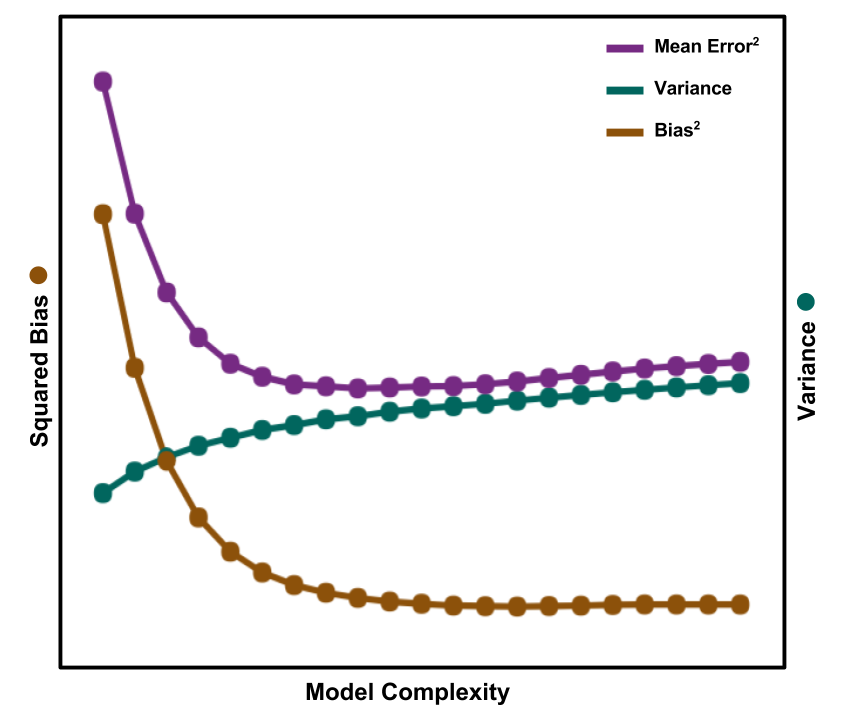
\includegraphics[width=\textwidth]{./chapters/litrev/BVtradeoff.png}}
  \caption{Bias and Variance Comprising Prediction Eror}
  \label{fig:bvtradeoff}
\end{figure}

As shown in Figure \ref{fig:bvtradeoff}, the shape of the total error curve
shows that there is a tradeoff between the bias and variance that can be
minimized. Some bias is desired in order to generalize to future unknown data.
But some variance is also positive for the model because it captures the
relationships in the data that the bias counteracts. 

\subsubsection{Types of Error}

While the sources of the model prediction error are well known, the creation of
a statistically learned model is a hidden process. Although the model emerges
from a black box, there are ways to evaluate the generalization (i.e.,
prediction) capability of it.  This is done by removing a small portion of the
data for use as a testing set.  The rest of the data set is known as the
training set and is used to train a model. After training, the test set is used
to test the model.  

The generalization error is typically referred to as the \textit{testing
error}, as it is measuring the ability of the model to predict future cases
that were not introduced in the training phase (i.e., the testing set entries).
Next, the \textit{training error} is provided by comparing the model
predictions to the training set, as the model would likely be smoother than the
potential noise the training set would include. This is useful to determine the
fitness of the model, the application of which is discussed below in Section
\ref{sec:optvalid}.

Although one could just train and test their model, there is a way to test the
model while still in the training phase. A testing set that would be used
during training to give feedback, a \textit{cross-validation} set, can provide
a faster convergence to a satisfactory model. As shown in Figure
\ref{fig:cverror}, this can be done by splitting the data set into three
groups: a large training set, a small cross-validation set, and a small testing
set. 

\begin{figure}[!htb]
  \centering
  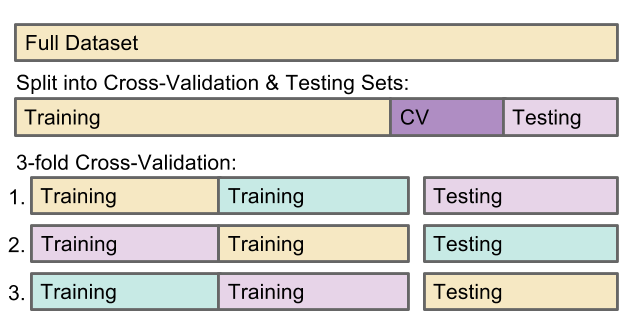
\includegraphics[width=0.85\linewidth]{./chapters/litrev/cverror.png}
  \caption{Illustration of Cross-Validation}
  \label{fig:cverror}
\end{figure}

However, in practice, multiple rounds of cross-validation steps are used,
referred to as \textit{k-fold cross-validation}. This allows a user to use all
data entries as a testing entry once.  As illustrated in Figure
\ref{fig:cverror}, this splits the dataset into \textit{k} subsets. One set is
designated as the testing set, and a model is trained with the rest. Following
the first training phase, another begins, this time with a different subset as
the testing set.  This process is performed \textit{k} times to give \textit{k}
models. The models are `averaged' by taking the mean of the predictions in the
case of regression or voting in the case of classification.  This provides an
additional level of model validation than can be achieved with a single testing
set.



\subsection{Model Optimization and Validation}
\label{sec:optvalid}
It is unlikely to have a model perform as one expects the first time. There are
therefore a few techniques for optimizing the performance. It should be noted
that much of the discussion here and in Section \ref{sec:valid} focuses on the
diagnostics aspect rather than the validation aspect of these techniques. In
practice, these are used for both purposes: diagnosing fitness problems and
proving good fitness.  But this work uses a formal comparison of model
performance for validation, introduced and detailed in Sections
\ref{sec:invcompare} and \ref{sec:modelcompare}, respectively. 

However, there is a risk associated with better prediction after using
optimization tools.  The increase in performance from over-optimization could
be linked to the training set performance and might not generalize outside of
the specific type of input data used.  A workaround for this scenario is to
obtain more data for the set or to obtain a completely different data set
altogether. 

\subsubsection{Training Set Size}

The first diagnostic plot for optimizing the model performance is called a
\textit{learning curve}, which provides information about the bias-variance
tradeoff with respect to the data set size. More specifically, learning curves
compare the training and cross-validation errors to the size of the training
set (i.e., number of instances in the training set). This is done by randomly
selecting a percentage of the the training set, inputting that into a
statistical learner, and tabulating the error of the learned model. 

Typically, a learning curve will look somewhat like one of the three examples
in Figure \ref{fig:learning}\footnote{These schematics are based on hand-drawn
diagrams by Ritchie Ng on http://www.ritchieng.com/applying-machine-learning/}.
A learning curve tests the model for high bias or high variance, which can
correspond to an under- or overfit model, respectively. 

\begin{figure}[!hp]
  \centering
  \begin{subfigure}[h]{0.65\linewidth}
    \centering
    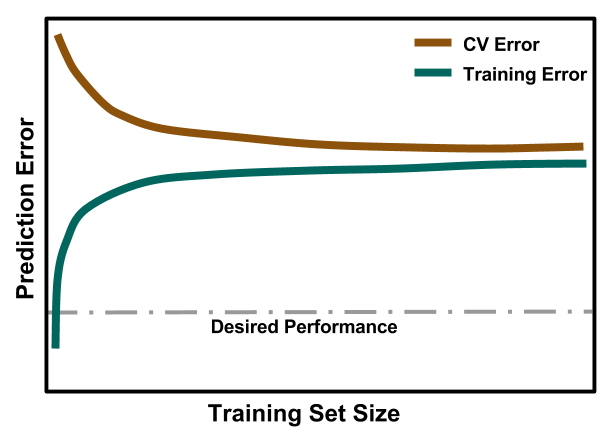
\includegraphics[width=\linewidth]{./chapters/litrev/LearningCurve-bias.png}
    \caption{High bias}
    \label{fig:bias}
  \end{subfigure}
  \begin{subfigure}[h]{0.65\linewidth}
    \centering
    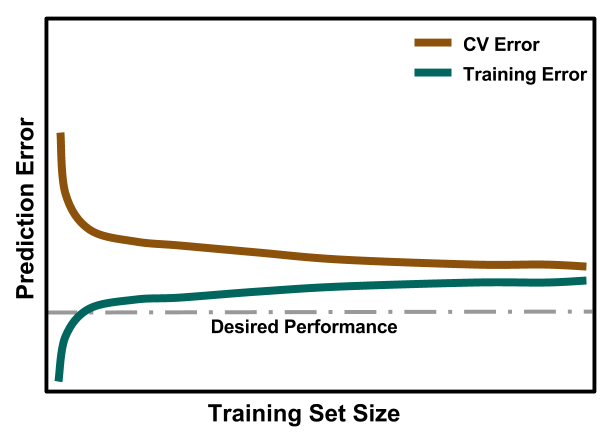
\includegraphics[width=\linewidth]{./chapters/litrev/LearningCurve-ideal.png}
    \caption{Ideal}
    \label{fig:ideal}
  \end{subfigure}
  \begin{subfigure}[h]{0.65\linewidth}
    \centering
    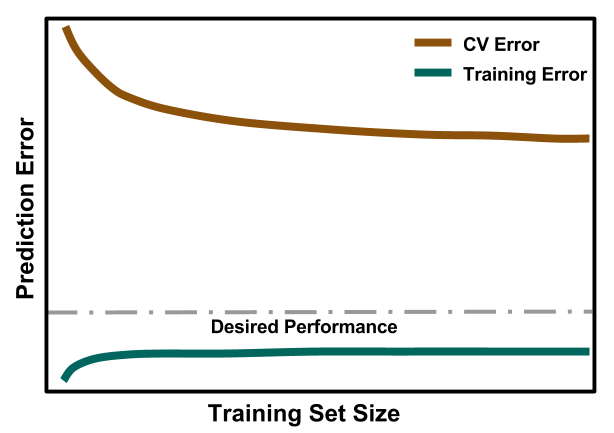
\includegraphics[width=\linewidth]{./chapters/litrev/LearningCurve-variance.png}
    \caption{High variance}
    \label{fig:variance}
  \end{subfigure}
  \caption{Learning Curves for Three Training Scenarios}
  \label{fig:learning}
\end{figure}

Figure \ref{fig:bias} suggests underfitting because the model is missing
important features in the data. It is characterized by a small gap between the
curves but high overall errors. The cross-validation error remains consistently
high and the training error increases drastically with increasing data, since
it is not generalizing well. 

Figure \ref{fig:variance} suggests overfitting because the model has too much
sensitivity to variations in the data. It is characterized by a very large gap
between the curves. It has an extremely low training error, as it has taken
into account every detail of the training set, but a high cross-validation
error because it cannot generalize beyond the testing set. 

Figure \ref{fig:ideal} is an example of a more ideal model fit. It is
characterized by a small gap between the two errors, and they are at a
reasonable level with respect to the desired performance.  The training error
should increase with respect to the training set size due to a larger amount of
bias (preventing overfitting). However, the cross-validation error should decrease
quickly with respect to the training set size due to being close to the minimum
of the bias-variance tradeoff. 

The training set size must be large and diverse enough to be considered
\gls{i.i.d.} because most \gls{ML} algorithms are developed upon this
assumption. Sometimes this is not possible, and the training data are skewed,
i.e., a portion of the data is over-represented. This must be handled
explicitly, but since each algorithm handles skewed data differently, it is
currently beyond the scope of this work. 

\subsubsection{Model Complexity}

After ensuring the appropriate training set size is selected, the models must
be further optimized using \textit{validation curves}.  These provide
information on the bias-variance tradeoff with respect to model complexity. Two
main tuneable factors affecting model complexity can cause the model to be
under- or overfit to the data: number of features in the data set and algorithm
parameters that control the regularization.

\begin{figure}[!htb]
  \centering
  \makebox[\textwidth][c]{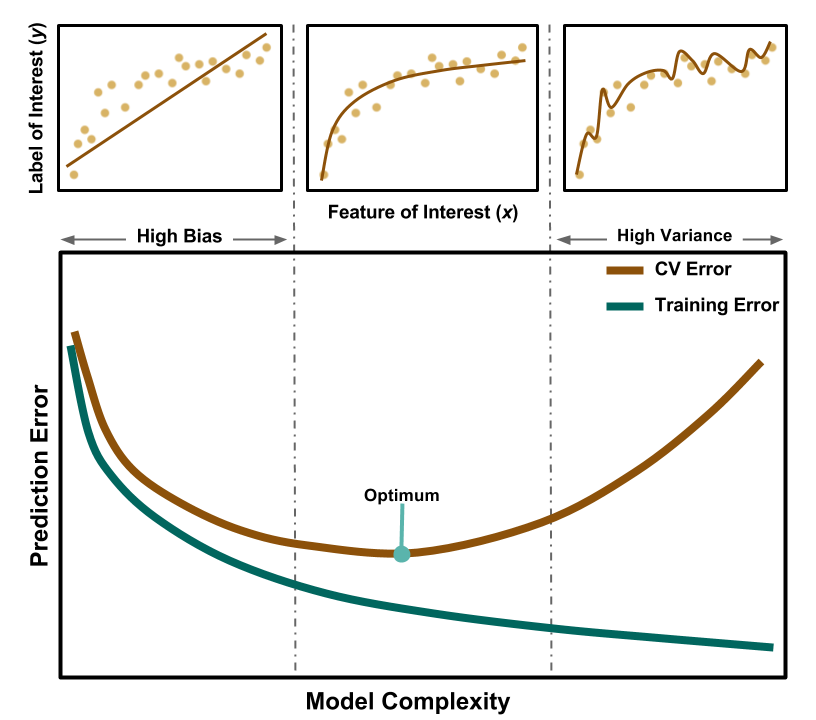
\includegraphics[width=1.2\textwidth]{./chapters/litrev/ValidationCurve.png}}
  \caption{Validation Curve with Different Model Fits}
  \label{fig:validation}
\end{figure}

Figure \ref{fig:validation} adapted from Ref. \cite{elements_stats} shows the
optimum as the minimum of the cross-validation error curve in the main (bottom)
plot. There is some gap between it and the training error, much larger than the
left side of the plot and much smaller than the right.  The top-middle plot is
a simplified visualization of an approximately well-fit model.  The left region
is marked by both errors being quite high, and above is an  illustration of how
an underfit plot (high bias) could provide high errors. The right region shows
the training error being quite low but the cross-validation error being high.
The diagram differing options with how to adjust to skewed training sets
\cite{scikit}.  above shows that it is obvious how the training error would be
negligible, but generalizing beyond that probably will not yield accurate
results. 

In practice, plotting learning and validation curves can be iterative. But as
previously mentioned, too many optimizations will result in a poorly performing
model when exposed to data outside of the training set.

\subsubsection{Comparison of Models}
\label{sec:invcompare}

In addition to evaluating a single learned model, it is beneficial to compare
models. Moreover, there are potential degeneracies in the solution space. This
is because most inverse problems are \textit{ill-posed}, because the solution
is not guaranteed to be unique \cite{skutnik_2016}.  Evaluating not only the
solution, but the confidence in the solution, is therefore prudent.

Both solution uncertainty and model comparison can be done using Bayesian
inference as discussed in Section \ref{sec:inverse}.  Equations \ref{eq:bayes}
and \ref{eq:bayes_words} show that there are three values to obtain to
calculate a posterior probability, i.e., the probability of a parameter
estimated from an \gls{ML} model being correct: likelihood, prior
probability, and marginal likelihood.  Comparing posterior probabilities among
different models reveal the most probable correct answer, i.e., the highest
posterior probability.  \cite{inverse_theory, gentle_bayes} Each of these
values are explained futher below.

The posterior probability represents the solution to an \textit{inverse}
problem, where model parameters are predicted from some given measurement
values. It is not directly computable and thus the remaining probabilities
discussed below indirectly allow its computation.  In this context, it is the
probability that a predicted reactor parameter from a chosen \gls{ML}
algorithm is correct given input based on an \gls{SNF} recipe.  For example, it
is the probability that a plutonium-239 concentration of $y\%$ is attributed to
a uranium oxide fuel in a \gls{BWR} with a burnup of $x\ GWd/MTU$.  

\begin{table}[!hp]
  \centering
  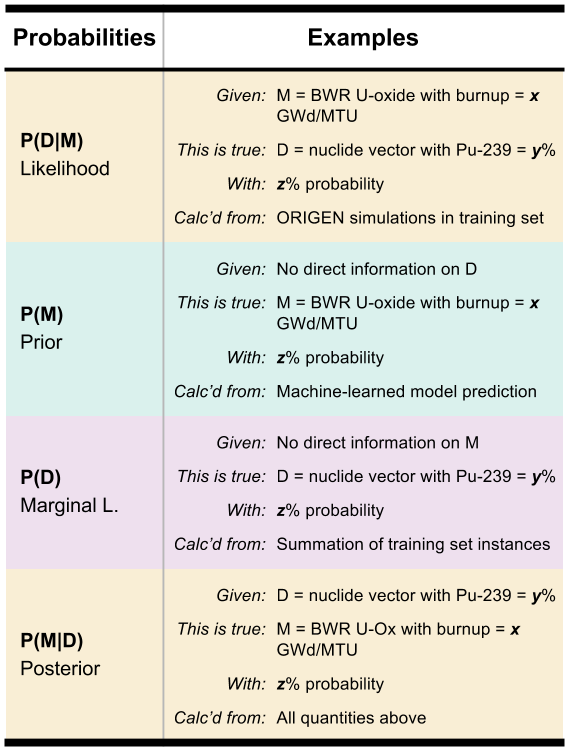
\includegraphics[width=\linewidth]{./chapters/litrev/bayes.png}
  \caption{Summary of Bayes Theorem Components}
  \label{tbl:bayes}
\end{table}

The prior probability represents the solution to a \textit{forward} problem,
where measurement values are predicted from some given model parameters.  In
this context, this is calculated from the instances in the training data set.
The likelihood is the probability that the output \gls{SNF} composition of a
simulation is correct given the input of reactor operation parameters.  In
practice, it will be calculated from a large number of forward simulations
using \gls{ORIGEN}, i.e., the training data set. For example, this would be the
probability that uranium oxide fuel from a \gls{BWR} having a burnup of $x\
GWd/MTU$ contains $y\%$ of plutonium-239.

The likelihood represents the spread of plausible \textit{model parameters}, so
it is a hypothesis based on the breadth of the model space with no evidence
provided.  In other words, it is given by model parametertization from a number
of potential sources.  One method is expert-elicited values.  Another is a
predicted model from some established theory or previously known relationship,
e.g., empirical relations between isotopic ratios and certain reactor
parameters or a direct calculation of the reactor parameters. In this context,
it is obtained from the estimated model parameters from a given statistical
model.  For example, it is the probability that a model from \gls{SVR} predicts
a burnup of $x\ GWd/MTU$ for uranium oxide fuel from a \gls{BWR} with no other
direct measurements provided.

The marginal likelihood represents the spread of plausible
\textit{measurements}, so it is based on the breath of the data space with no
model-based information provided.  In practice, however, it is calculated by
summing the joint probabilities of all possible model parameter hypotheses and
measurements. This in essence provides a normalization constant for the Bayes'
equation.  Thus, the marginal likelihood is only needed for absolute posterior
probability calculations; it does not affect the relative probabilities, which
are all that is needed for model comparison. \cite{inverse_theory,
bayes_compare}

For reference, Table \ref{tbl:bayes} is a summary of the Bayes' theorem
components described above as related to this work. In the table, \textbf{P} is
a probability, \textbf{D} is a set of measurements (i.e., data), and \textbf{M}
is a set of model parameters. The examples used in the discussion above are
reiterated here.


